% Created by tikzDevice version 0.7.0 on 2014-04-28 15:35:22
% !TEX encoding = UTF-8 Unicode
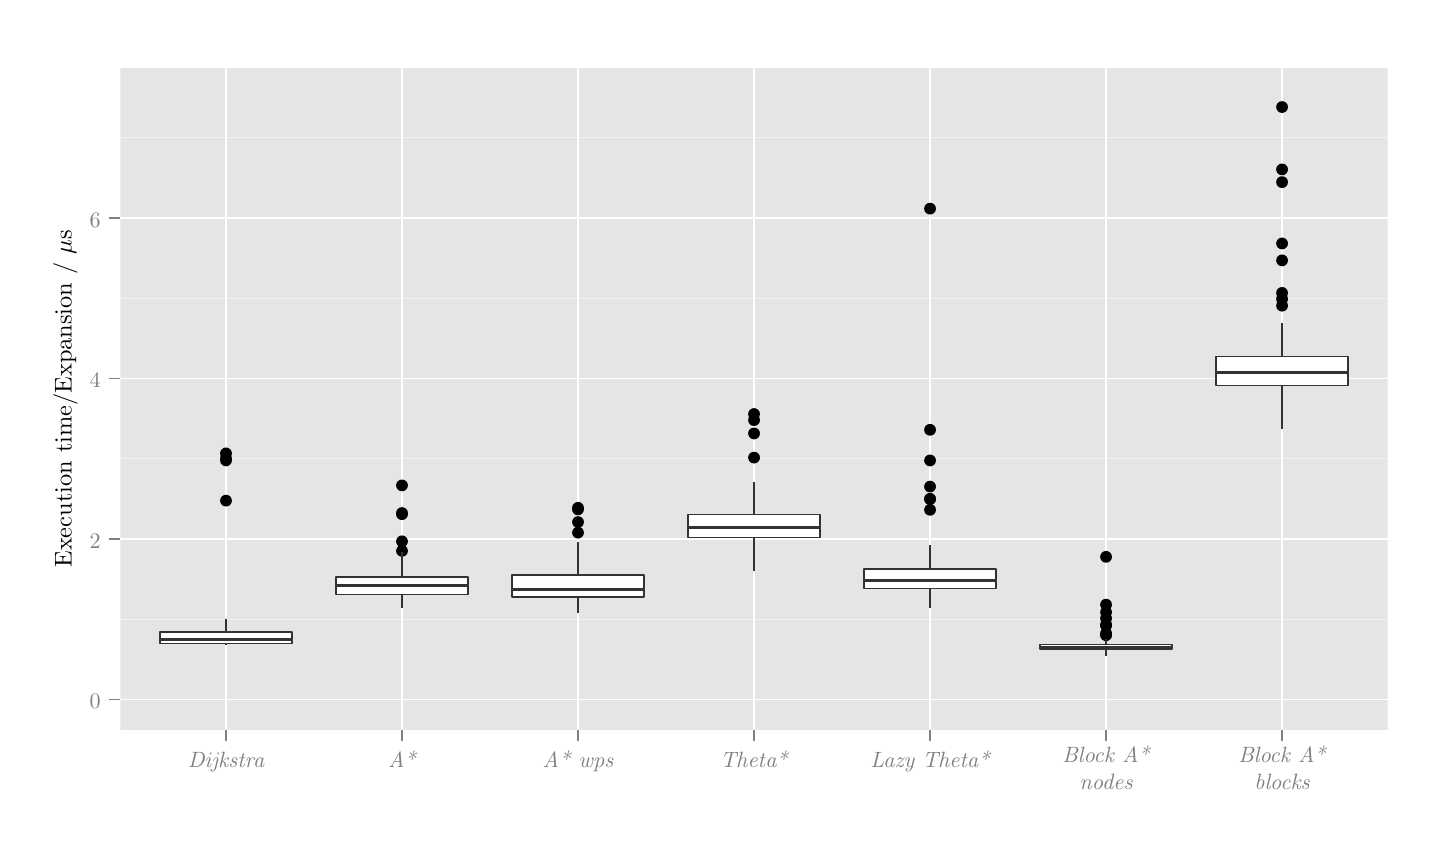
\begin{tikzpicture}[x=1pt,y=1pt]
\definecolor[named]{fillColor}{rgb}{1.00,1.00,1.00}
\path[use as bounding box,fill=fillColor,fill opacity=0.00] (0,0) rectangle (505.89,289.08);
\begin{scope}
\path[clip] (  0.00,  0.00) rectangle (505.89,289.08);
\definecolor[named]{drawColor}{rgb}{1.00,1.00,1.00}
\definecolor[named]{fillColor}{rgb}{1.00,1.00,1.00}

\path[draw=drawColor,line width= 0.6pt,line join=round,line cap=round,fill=fillColor] (  0.00, -0.00) rectangle (505.89,289.08);
\end{scope}
\begin{scope}
\path[clip] ( 33.50, 35.41) rectangle (491.44,274.63);
\definecolor[named]{fillColor}{rgb}{0.90,0.90,0.90}

\path[fill=fillColor] ( 33.50, 35.41) rectangle (491.44,274.63);
\definecolor[named]{drawColor}{rgb}{0.95,0.95,0.95}

\path[draw=drawColor,line width= 0.3pt,line join=round] ( 33.50, 75.28) --
	(491.44, 75.28);

\path[draw=drawColor,line width= 0.3pt,line join=round] ( 33.50,133.27) --
	(491.44,133.27);

\path[draw=drawColor,line width= 0.3pt,line join=round] ( 33.50,191.26) --
	(491.44,191.26);

\path[draw=drawColor,line width= 0.3pt,line join=round] ( 33.50,249.25) --
	(491.44,249.25);
\definecolor[named]{drawColor}{rgb}{1.00,1.00,1.00}

\path[draw=drawColor,line width= 0.6pt,line join=round] ( 33.50, 46.28) --
	(491.44, 46.28);

\path[draw=drawColor,line width= 0.6pt,line join=round] ( 33.50,104.28) --
	(491.44,104.28);

\path[draw=drawColor,line width= 0.6pt,line join=round] ( 33.50,162.27) --
	(491.44,162.27);

\path[draw=drawColor,line width= 0.6pt,line join=round] ( 33.50,220.26) --
	(491.44,220.26);

\path[draw=drawColor,line width= 0.6pt,line join=round] ( 71.66, 35.41) --
	( 71.66,274.63);

\path[draw=drawColor,line width= 0.6pt,line join=round] (135.26, 35.41) --
	(135.26,274.63);

\path[draw=drawColor,line width= 0.6pt,line join=round] (198.86, 35.41) --
	(198.86,274.63);

\path[draw=drawColor,line width= 0.6pt,line join=round] (262.47, 35.41) --
	(262.47,274.63);

\path[draw=drawColor,line width= 0.6pt,line join=round] (326.07, 35.41) --
	(326.07,274.63);

\path[draw=drawColor,line width= 0.6pt,line join=round] (389.67, 35.41) --
	(389.67,274.63);

\path[draw=drawColor,line width= 0.6pt,line join=round] (453.27, 35.41) --
	(453.27,274.63);
\definecolor[named]{fillColor}{rgb}{0.00,0.00,0.00}

\path[fill=fillColor] ( 71.66,133.43) circle (  2.13);

\path[fill=fillColor] ( 71.66,135.25) circle (  2.13);

\path[fill=fillColor] ( 71.66,118.17) circle (  2.13);

\path[fill=fillColor] ( 71.66,132.70) circle (  2.13);
\definecolor[named]{drawColor}{rgb}{0.20,0.20,0.20}
\definecolor[named]{fillColor}{rgb}{0.20,0.20,0.20}

\path[draw=drawColor,line width= 0.6pt,line join=round,fill=fillColor] ( 71.66, 70.63) -- ( 71.66, 75.53);

\path[draw=drawColor,line width= 0.6pt,line join=round,fill=fillColor] ( 71.66, 66.60) -- ( 71.66, 65.91);
\definecolor[named]{fillColor}{rgb}{1.00,1.00,1.00}

\path[draw=drawColor,line width= 0.6pt,line join=round,line cap=round,fill=fillColor] ( 47.81, 70.63) --
	( 47.81, 66.60) --
	( 95.51, 66.60) --
	( 95.51, 70.63) --
	( 47.81, 70.63) --
	cycle;
\definecolor[named]{fillColor}{rgb}{0.20,0.20,0.20}

\path[draw=drawColor,line width= 1.1pt,line join=round,fill=fillColor] ( 47.81, 67.90) -- ( 95.51, 67.90);
\definecolor[named]{fillColor}{rgb}{0.00,0.00,0.00}

\path[fill=fillColor] (135.26,123.68) circle (  2.13);

\path[fill=fillColor] (135.26,113.27) circle (  2.13);

\path[fill=fillColor] (135.26,113.69) circle (  2.13);

\path[fill=fillColor] (135.26,100.03) circle (  2.13);

\path[fill=fillColor] (135.26,103.47) circle (  2.13);
\definecolor[named]{fillColor}{rgb}{0.20,0.20,0.20}

\path[draw=drawColor,line width= 0.6pt,line join=round,fill=fillColor] (135.26, 90.50) -- (135.26, 99.61);

\path[draw=drawColor,line width= 0.6pt,line join=round,fill=fillColor] (135.26, 84.23) -- (135.26, 79.42);
\definecolor[named]{fillColor}{rgb}{1.00,1.00,1.00}

\path[draw=drawColor,line width= 0.6pt,line join=round,line cap=round,fill=fillColor] (111.41, 90.50) --
	(111.41, 84.23) --
	(159.11, 84.23) --
	(159.11, 90.50) --
	(111.41, 90.50) --
	cycle;
\definecolor[named]{fillColor}{rgb}{0.20,0.20,0.20}

\path[draw=drawColor,line width= 1.1pt,line join=round,fill=fillColor] (111.41, 87.43) -- (159.11, 87.43);
\definecolor[named]{fillColor}{rgb}{0.00,0.00,0.00}

\path[fill=fillColor] (198.86,110.43) circle (  2.13);

\path[fill=fillColor] (198.86,115.58) circle (  2.13);

\path[fill=fillColor] (198.86,115.00) circle (  2.13);

\path[fill=fillColor] (198.86,106.60) circle (  2.13);
\definecolor[named]{fillColor}{rgb}{0.20,0.20,0.20}

\path[draw=drawColor,line width= 0.6pt,line join=round,fill=fillColor] (198.86, 91.31) -- (198.86,103.15);

\path[draw=drawColor,line width= 0.6pt,line join=round,fill=fillColor] (198.86, 83.27) -- (198.86, 77.65);
\definecolor[named]{fillColor}{rgb}{1.00,1.00,1.00}

\path[draw=drawColor,line width= 0.6pt,line join=round,line cap=round,fill=fillColor] (175.01, 91.31) --
	(175.01, 83.27) --
	(222.72, 83.27) --
	(222.72, 91.31) --
	(175.01, 91.31) --
	cycle;
\definecolor[named]{fillColor}{rgb}{0.20,0.20,0.20}

\path[draw=drawColor,line width= 1.1pt,line join=round,fill=fillColor] (175.01, 86.03) -- (222.72, 86.03);
\definecolor[named]{fillColor}{rgb}{0.00,0.00,0.00}

\path[fill=fillColor] (262.47,149.47) circle (  2.13);

\path[fill=fillColor] (262.47,147.28) circle (  2.13);

\path[fill=fillColor] (262.47,133.72) circle (  2.13);

\path[fill=fillColor] (262.47,142.44) circle (  2.13);
\definecolor[named]{fillColor}{rgb}{0.20,0.20,0.20}

\path[draw=drawColor,line width= 0.6pt,line join=round,fill=fillColor] (262.47,113.19) -- (262.47,124.78);

\path[draw=drawColor,line width= 0.6pt,line join=round,fill=fillColor] (262.47,104.80) -- (262.47, 92.67);
\definecolor[named]{fillColor}{rgb}{1.00,1.00,1.00}

\path[draw=drawColor,line width= 0.6pt,line join=round,line cap=round,fill=fillColor] (238.62,113.19) --
	(238.62,104.80) --
	(286.32,104.80) --
	(286.32,113.19) --
	(238.62,113.19) --
	cycle;
\definecolor[named]{fillColor}{rgb}{0.20,0.20,0.20}

\path[draw=drawColor,line width= 1.1pt,line join=round,fill=fillColor] (238.62,108.46) -- (286.32,108.46);
\definecolor[named]{fillColor}{rgb}{0.00,0.00,0.00}

\path[fill=fillColor] (326.07,143.77) circle (  2.13);

\path[fill=fillColor] (326.07,132.69) circle (  2.13);

\path[fill=fillColor] (326.07,123.25) circle (  2.13);

\path[fill=fillColor] (326.07,114.86) circle (  2.13);

\path[fill=fillColor] (326.07,118.84) circle (  2.13);

\path[fill=fillColor] (326.07,118.70) circle (  2.13);

\path[fill=fillColor] (326.07,223.69) circle (  2.13);
\definecolor[named]{fillColor}{rgb}{0.20,0.20,0.20}

\path[draw=drawColor,line width= 0.6pt,line join=round,fill=fillColor] (326.07, 93.48) -- (326.07,102.19);

\path[draw=drawColor,line width= 0.6pt,line join=round,fill=fillColor] (326.07, 86.40) -- (326.07, 79.45);
\definecolor[named]{fillColor}{rgb}{1.00,1.00,1.00}

\path[draw=drawColor,line width= 0.6pt,line join=round,line cap=round,fill=fillColor] (302.22, 93.48) --
	(302.22, 86.40) --
	(349.92, 86.40) --
	(349.92, 93.48) --
	(302.22, 93.48) --
	cycle;
\definecolor[named]{fillColor}{rgb}{0.20,0.20,0.20}

\path[draw=drawColor,line width= 1.1pt,line join=round,fill=fillColor] (302.22, 89.42) -- (349.92, 89.42);
\definecolor[named]{fillColor}{rgb}{0.00,0.00,0.00}

\path[fill=fillColor] (389.67, 97.86) circle (  2.13);

\path[fill=fillColor] (389.67, 70.25) circle (  2.13);

\path[fill=fillColor] (389.67, 80.59) circle (  2.13);

\path[fill=fillColor] (389.67, 77.87) circle (  2.13);

\path[fill=fillColor] (389.67, 75.66) circle (  2.13);

\path[fill=fillColor] (389.67, 69.72) circle (  2.13);

\path[fill=fillColor] (389.67, 73.01) circle (  2.13);

\path[fill=fillColor] (389.67, 73.33) circle (  2.13);

\path[fill=fillColor] (389.67, 69.54) circle (  2.13);
\definecolor[named]{fillColor}{rgb}{0.20,0.20,0.20}

\path[draw=drawColor,line width= 0.6pt,line join=round,fill=fillColor] (389.67, 66.21) -- (389.67, 68.13);

\path[draw=drawColor,line width= 0.6pt,line join=round,fill=fillColor] (389.67, 64.45) -- (389.67, 61.93);
\definecolor[named]{fillColor}{rgb}{1.00,1.00,1.00}

\path[draw=drawColor,line width= 0.6pt,line join=round,line cap=round,fill=fillColor] (365.82, 66.21) --
	(365.82, 64.45) --
	(413.52, 64.45) --
	(413.52, 66.21) --
	(365.82, 66.21) --
	cycle;
\definecolor[named]{fillColor}{rgb}{0.20,0.20,0.20}

\path[draw=drawColor,line width= 1.1pt,line join=round,fill=fillColor] (365.82, 65.18) -- (413.52, 65.18);
\definecolor[named]{fillColor}{rgb}{0.00,0.00,0.00}

\path[fill=fillColor] (453.27,191.04) circle (  2.13);

\path[fill=fillColor] (453.27,260.40) circle (  2.13);

\path[fill=fillColor] (453.27,237.86) circle (  2.13);

\path[fill=fillColor] (453.27,233.27) circle (  2.13);

\path[fill=fillColor] (453.27,188.62) circle (  2.13);

\path[fill=fillColor] (453.27,204.99) circle (  2.13);

\path[fill=fillColor] (453.27,211.10) circle (  2.13);

\path[fill=fillColor] (453.27,193.23) circle (  2.13);
\definecolor[named]{fillColor}{rgb}{0.20,0.20,0.20}

\path[draw=drawColor,line width= 0.6pt,line join=round,fill=fillColor] (453.27,170.29) -- (453.27,182.48);

\path[draw=drawColor,line width= 0.6pt,line join=round,fill=fillColor] (453.27,159.83) -- (453.27,144.21);
\definecolor[named]{fillColor}{rgb}{1.00,1.00,1.00}

\path[draw=drawColor,line width= 0.6pt,line join=round,line cap=round,fill=fillColor] (429.42,170.29) --
	(429.42,159.83) --
	(477.13,159.83) --
	(477.13,170.29) --
	(429.42,170.29) --
	cycle;
\definecolor[named]{fillColor}{rgb}{0.20,0.20,0.20}

\path[draw=drawColor,line width= 1.1pt,line join=round,fill=fillColor] (429.42,164.55) -- (477.13,164.55);
\end{scope}
\begin{scope}
\path[clip] (  0.00,  0.00) rectangle (505.89,289.08);
\definecolor[named]{drawColor}{rgb}{0.50,0.50,0.50}

\node[text=drawColor,anchor=base east,inner sep=0pt, outer sep=0pt, scale=  0.80] at ( 26.38, 42.98) {0};

\node[text=drawColor,anchor=base east,inner sep=0pt, outer sep=0pt, scale=  0.80] at ( 26.38,100.97) {2};

\node[text=drawColor,anchor=base east,inner sep=0pt, outer sep=0pt, scale=  0.80] at ( 26.38,158.96) {4};

\node[text=drawColor,anchor=base east,inner sep=0pt, outer sep=0pt, scale=  0.80] at ( 26.38,216.95) {6};
\end{scope}
\begin{scope}
\path[clip] (  0.00,  0.00) rectangle (505.89,289.08);
\definecolor[named]{drawColor}{rgb}{0.50,0.50,0.50}

\path[draw=drawColor,line width= 0.6pt,line join=round] ( 29.23, 46.28) --
	( 33.50, 46.28);

\path[draw=drawColor,line width= 0.6pt,line join=round] ( 29.23,104.28) --
	( 33.50,104.28);

\path[draw=drawColor,line width= 0.6pt,line join=round] ( 29.23,162.27) --
	( 33.50,162.27);

\path[draw=drawColor,line width= 0.6pt,line join=round] ( 29.23,220.26) --
	( 33.50,220.26);
\end{scope}
\begin{scope}
\path[clip] (  0.00,  0.00) rectangle (505.89,289.08);
\definecolor[named]{drawColor}{rgb}{0.50,0.50,0.50}

\path[draw=drawColor,line width= 0.6pt,line join=round] ( 71.66, 31.14) --
	( 71.66, 35.41);

\path[draw=drawColor,line width= 0.6pt,line join=round] (135.26, 31.14) --
	(135.26, 35.41);

\path[draw=drawColor,line width= 0.6pt,line join=round] (198.86, 31.14) --
	(198.86, 35.41);

\path[draw=drawColor,line width= 0.6pt,line join=round] (262.47, 31.14) --
	(262.47, 35.41);

\path[draw=drawColor,line width= 0.6pt,line join=round] (326.07, 31.14) --
	(326.07, 35.41);

\path[draw=drawColor,line width= 0.6pt,line join=round] (389.67, 31.14) --
	(389.67, 35.41);

\path[draw=drawColor,line width= 0.6pt,line join=round] (453.27, 31.14) --
	(453.27, 35.41);
\end{scope}
\begin{scope}
\path[clip] (  0.00,  0.00) rectangle (505.89,289.08);
\definecolor[named]{drawColor}{rgb}{0.50,0.50,0.50}

\node[text=drawColor,anchor=base,inner sep=0pt, outer sep=0pt, scale=  0.80] at ( 71.66, 21.69) {{\em Dijkstra}};

\node[text=drawColor,anchor=base,inner sep=0pt, outer sep=0pt, scale=  0.80] at (135.26, 21.69) {{\em A*}};

\node[text=drawColor,anchor=base,inner sep=0pt, outer sep=0pt, scale=  0.80] at (198.86, 21.69) {{\em A* wps}};

\node[text=drawColor,anchor=base,inner sep=0pt, outer sep=0pt, scale=  0.80] at (262.47, 21.69) {{\em Theta*}};

\node[text=drawColor,anchor=base,inner sep=0pt, outer sep=0pt, scale=  0.80] at (326.07, 21.69) {{\em Lazy Theta*}};

\node[text=drawColor,inner sep=0pt, outer sep=0pt, scale=  0.80, align=center] at (389.67, 21.69) {{\em Block A*}\\{\em nodes}};

\node[text=drawColor,inner sep=0pt, outer sep=0pt, scale=  0.80,align=center] at (453.27, 21.69) {{\em Block A*}\\{\em blocks}};
\end{scope}
\begin{scope}
\path[clip] (  0.00,  0.00) rectangle (505.89,289.08);
\definecolor[named]{drawColor}{rgb}{0.00,0.00,0.00}

\node[text=drawColor,rotate= 90.00,anchor=base,inner sep=0pt, outer sep=0pt, scale=  0.88] at ( 15.90,155.02) {Execution time/Expansion / $\mu$s};
\end{scope}
\end{tikzpicture}
